% !TEX root = ..\main.tex
\chapter{Introduction}

\section{Motivation and background}
Today, hardware and software based systems, further known as embedded systems, are growing rapidly. Ranging from microprosessors in cellphones to sensors in cars and surveillance systems, embedded computing is becoming a big part of our lives. With the rapid growth of embedded systems, we clearly see that most future computing systems will be embedded systems\cite{wolfmadsen-2000}. With the new era of Internet of Things, more and more embedded systems are getting a networked interconnection. This leads to a distributed network of devices communicating with other devices as well as human beings. Gartner has estimated that in 2020, 25 billion connected "things" will be in use\cite{gartner}. To provide more functionality, multiple components are combined together with embedded systems. However, as the complexity of embedded system increases, the ability to maintain the quality of such systems becomes more difficult. Combination of multiple components leads to higher costs of verifying additional software and many fails to test the product properly and deliver a reliable product. Such systems accumulates technical debt. As debt accumulates, it becomes necessary to manage the overall debt while keeping the system flexible and extensible. Companies must often recall their products. If they could catch these software defects earlier in the system design process, they would have saved a lot of money. Embedded systems also has long lifetime and its important to find out how to make decisisions so future maintenance and evolution has low cost as possible. 

With the rapid evolution of electrical and software based systems, known as embedded systems, we see that most of the future compuing systems will be embedded systems\cite{wolfmadsen-2000}. However, as the complexity of embedded systems increases, maintaining the quality of such systems becomes more difficult. Higher functionality is provided when multiple components are combined together with embedde systems. This type of combination leads to higher cost of verifying additional software, which makes many fail to test the product properly and deliver reliable products. Companies must often recall their products, and catching these software defects earlier in the system design process saves a lot of money. The ability to identify these kind of problems earlier is still something many companies has troubles with. Embedded systems has also long lifetime and it's important to find out how to make decisions so future maintenance and operation has low cost as possible. Technical debt is a big factor in embedded systems as developers might not be available years after implementaion. 

Since embedded systems are some specialized hardware,

\begin{table}
	\centering
	\begin{tabular}{ | l | l | l | l | l |}
	\hline
	\textbf{Category} & \textbf{2013} & \textbf{2014} & \textbf{2015} & \textbf{2020} \\ \hline
	Automotive & 96.0 & 189.6 & 372.3 & 3,511.1 \\ \hline
	Consumer & 1,842.1 & 2,244.5 & 2,874.9 & 13,172.5 \\ \hline
	Generic Business & 395.2 & 479.4 & 623.9 & 5,158.6 \\ \hline
	Vertical Business & 698.7 & 836.5 & 1,009.4 & 3,164.4 \\ \hline
	\textbf{Grand Total} & \textbf{3,032.0} & \textbf{3,750.0} & \textbf{4,880.6} & \textbf{25,006.6} \\
	\hline
	\end{tabular}
	\caption{Table from Gartner\cite{gartner}} \label{tab:table1}
\end{table}

Technical debt is a rising problem. It is estimated that the cost of dealing with technical debt threatens to grow to \$ 1 trillion globally by 2015\cite{gartner2010}. That is the double of the amount technical debt in 2010. IT management teams must measure the level of technical debt in their organization and develop a strategy to deal with it.


\section{Research Questions}
The main objective of this project is to increase the knowledge on how the significant sources of technical debt, and find out how technical debt in embedded systems are managed. The reason for this is that embedded systems usually has long lifetime, and it is important to find out how such systems are managed because the architecture and design decisions are usually made long time ago and these people might not be available. 

\textbf{The research questions will be:} 
\begin{itemize}
	\item \textbf{RQ-1}: Are there any practices and tools for managing technical debt? How are they used?
	\item \textbf{RQ-2}: What are the most significant sources of technical debt?
	\item \textbf{RQ-3}: When should a debt be refactored?
	\item \textbf{RQ-4}: Who is responsible for deciding whether to incur, and pay off technical debt?
\end{itemize}

\section{Research method}
The most relevant research methologies in software engineering is summarized in Figure \ref{fig:researchProcess}. This model will be used as a basis in this thesis. In order to define the research questions, it is necessary to an overview of the research field. To do this, one can either conduct a review of published research within the selected area of study, or use experiences and motivations. Following this, a research strategy is needed to answer the research questions. There are six different research strategies: survey, design and creation, experiment, case study, action research, and ethnography. To produce empirical data or evidence, a data generation method is needed. There are four methods: interviews, observations, questionnaire, and documents. These data can either be quantitative or qualitative. 

To achieve my goal, a litterature review will be conducted in order to get familiar with the area of study. Following this, one or more research questions will be defined. In order to answer the research questions, a series of semi-structured interviews is conducted with software developers and managers working with various systems. 

\begin{figure}
	\centering
	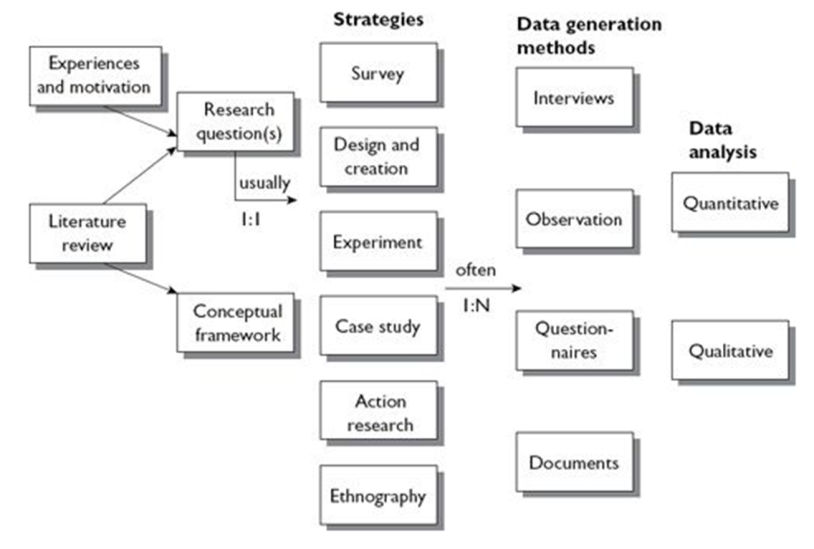
\includegraphics[width=0.8\textwidth]{images/researchStrategies.png}
	\caption{Model of research process\cite{Oates:2006:RIS:1202299}}
	\label{fig:researchProcess}
\end{figure}

\section{Project structure}
The report is structured as follows:

\begin{itemize}
	\item \textbf{Chapter 1} introduces the problem and motivation behind this project, the research questions and the different parts of this project.
	\item \textbf{Chapter 2} provides state-of-art within the field of techincal debt, embedded systems, and software engineering.
	\item \textbf{Chapter 3} presents the research method, and the procedures behind the method.
	\item \textbf{Chapter 4} provides an overview of the results and analyses from the research method.
	\item \textbf{Chapter 5} presents a discussion of the whole project.
	\item \textbf{Chapter 6} concludes the report and provides some points to future work. 
\end{itemize}

